\documentclass{oxmathproblems}
\usepackage{blindtext}
\usepackage{hyperref}
\usepackage{geometry}

\course{ITAM - Estadística 1}
\oxfordterm{ Solución Assignment 01}
\sheetnumber{1}
\sheettitle{}

\begin{document}
\begin{questions}
\miquestion \textbf{Datos Cualitativos y distribuciones de frecuencia}

\begin{itemize}
\item  a) Cualitativo/ Nominal 
\item  b) Cuantitativo / Razón
\item  c) Cualitativa / Nominal 
\item  d) Cuantitativa / Intervalo
\item  e) Cuantitativa / Razón
\end{itemize}

\miquestion \textbf {Distribución de frecuencias y Diagrama de puntos}

\begin{itemize}
\item  a) Histograma: 
$$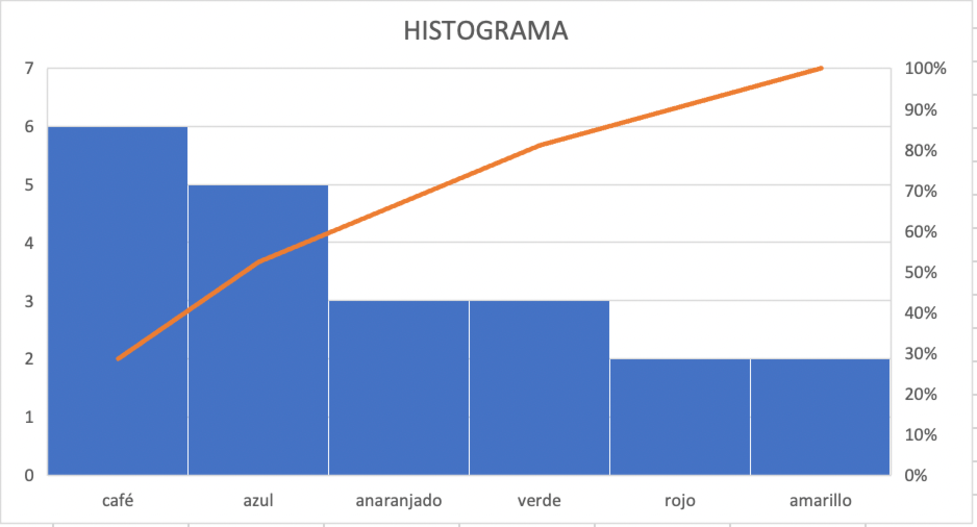
\includegraphics[width=0.8\textwidth]{Histcolor}$$
\item  b) Diagrama de Puntos: 
$$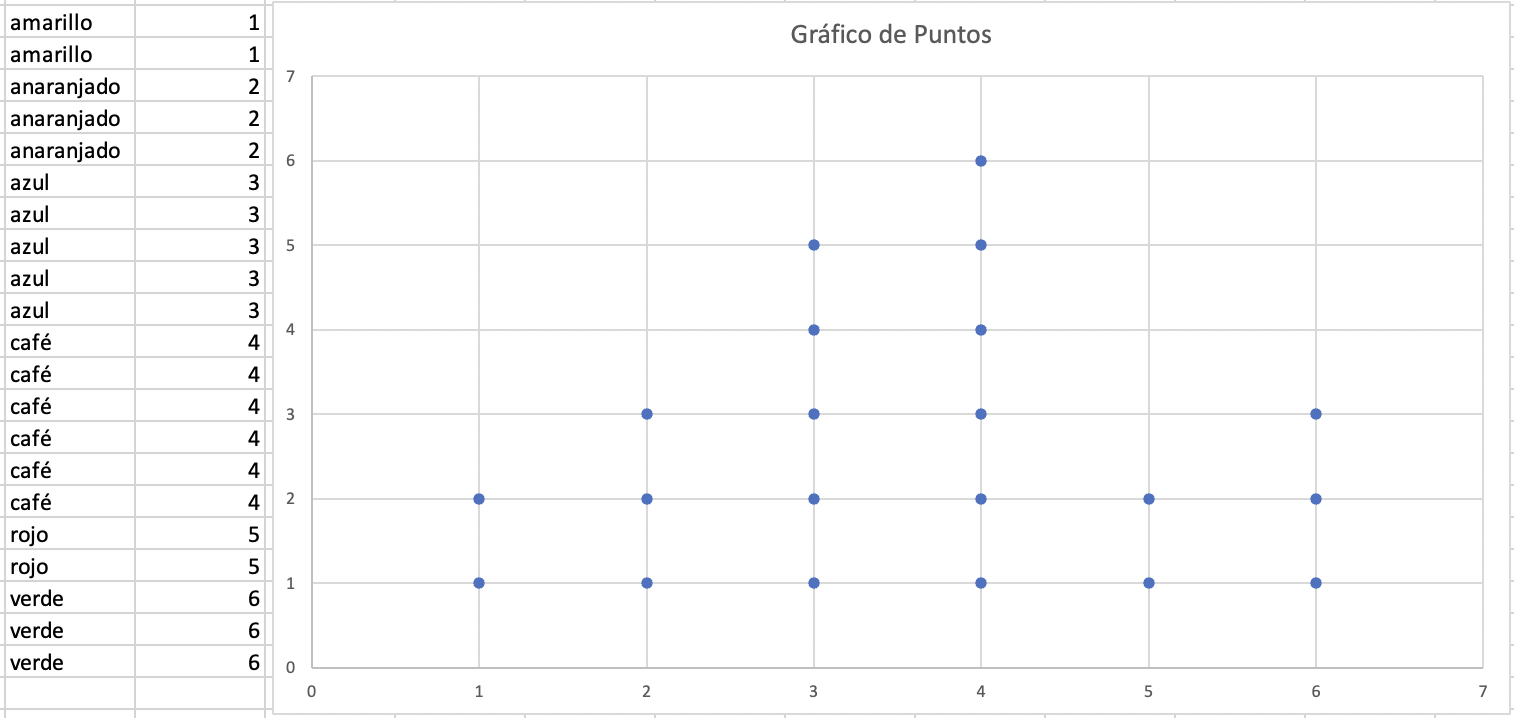
\includegraphics[width=0.8\textwidth]{Diagramapunto}$$
\item  c) Tabla de distribución de frecuencias: 
\begin{center}
\begin{tabular}{ |c|c|c|c|c|c|c|} 
\hline
Variable Cualitativa & Frecuencia Absoluta & Frec relativa & Frecuencia Acum & Frec Acum Relat   \\
\hline
Amarillo &2 &0.095 & 2 & 0.095\\
Anaranjado &3& 0.143 & 5 & 0.238\\
Azul  & 5  & 0.238  & 10 & 0.476\\
Café & 6 & 0.286 &  16 &0.761\\
Rojo & 2 & 0.095 & 18 & 0.857\\
Verde & 3 & 0.143 & 21 & 1 \\
Total & 21 & 1 &- & - \\
\hline
\end{tabular}
\end{center}

\end{itemize}

\miquestion \textbf { Diagrama de Tallo y Hoja} 

4$\mid$ 0 

6$\mid$ 0 5 5 5 8 8 

7$\mid$ 0 0 0 0 0 0 0 

7$\mid$4  5 5 

9$\mid$ 0 5 

\text  {siendo} 9$\mid$ 0 \text  { como   90}




\end{questions}




\end{document}
